\RequirePackage{currfile}
\documentclass[]{beamer}
\usepackage{verbatim}
\usepackage{standalone}
\usepackage{graphicx}
\graphicspath{{../figs/}}

\usepackage{ amssymb }
\usepackage{amsmath}
\usepackage{multirow}

\usepackage{cancel}
\usepackage{rotating}


%%%%%%%%%%%%%%%%%%%%%% misc
\newcommand{\iitem}[1]{\begin{itemize}
		\item #1
	\end{itemize}}


%%%%%%%%%%%%%%%%%%%%%%%%%%
% PGFPLOTS
\usepackage{pgfplots}
\pgfplotsset{compat=1.12}
\usepackage{booktabs, array} % Generates table from .csv
\usepackage{pgfplotstable}

\newcolumntype{C}[1]{>{\centering\arraybackslash}m{#1}}

\pgfplotstableset{percent style/.style=}
		}},
		%
		%
		every head row/.style={after row=\midrule},
	}
	
\pgfplotsset{width=0.9\textwidth,height=0.6\textwidth}
	
%%%%%%%%%%%%%%%%%%%


\usepackage{arrayjobx}
\usepackage{xifthen}
\usepackage{tikz,textcomp}
\usetikzlibrary{positioning}
\newcommand{\fullpagetikz}[1]{{\input{#1}}}
\newcommand{\widthtikz}[2]{\resizebox{#1\textwidth}{!}{\input{#2}}}
\newcommand{\fullwidthtikz}[1]{\resizebox{0.9\textwidth}{!}{\input{#1}}}

%%%%%%%%%%%%%Bibliography
\usepackage[backend=bibtex, url=false,
bibstyle=ieee,firstinits=true]{biblatex}
\bibliography{master.bib}
\renewcommand*{\thefootnote}{} %No symbol or marker
\renewcommand{\footnotesize}{\scriptsize}
%%%%%%%%%%%%%%%%%


\usepackage{xcolor}
\definecolor{chamois}{RGB}{255,255,240}
\definecolor{darkbrown}{RGB}{124,79,0}
\definecolor{UniBlue}{RGB}{83,101,130}

\definecolor{hellgelb}{rgb}{1,1,0.8}
\definecolor{colKeys}{rgb}{0,0,1}
\definecolor{colIdentifier}{rgb}{0,0,0}
\definecolor{colComments}{rgb}{1,0,0}
\definecolor{colString}{rgb}{0,0.5,0}

\usefonttheme{professionalfonts}
\usepackage{tgadventor}
\renewcommand*\familydefault{\sfdefault}
\usepackage[T1]{fontenc}
\usepackage{microtype}


\newcommand{\topline}{%
  \tikz[remember picture,overlay] {%
    \draw[brown,ultra thick] ([yshift=-1.8cm]current page.north west)-- ([yshift=-1.8cm,xshift=\paperwidth]current page.north west);} }

\renewcommand{\topline}{}

\setbeamertemplate{frametitle}{\begin{minipage}[b][1.8cm][c]{\textwidth}%
	\centering%
	\insertframetitle\\\insertframesubtitle
	\end{minipage}}
	

\addtobeamertemplate{frametitle}{}{\topline%
}

\setbeamertemplate{navigation symbols}{}
\setbeamercolor{background canvas}{bg=chamois}
\setbeamercolor{itemize item}{fg=brown}
%\setbeamertemplate{itemize item}{\maltese}
\setbeamercolor{itemize subitem}{fg=brown}
%\setbeamertemplate{itemize subitem}{\begin{rotate}{90}$\diamondsuit$\end{rotate}}

\setbeamercolor{title}{fg=UniBlue}
\setbeamercolor{frametitle}{fg=UniBlue}    
\setbeamerfont{frametitle}{size=\Large}

\setbeamercolor{author}{fg=darkbrown}
\setbeamercolor{institute}{fg=darkbrown}
\setbeamercolor{date}{fg=darkbrown}


\setbeamercolor{structure}{fg=UniBlue}
\setbeamercolor{alerted text}{fg=UniBlue}
\setbeamercolor{alerted text}{fg=UniBlue}
\setbeamercolor{normal text}{fg=darkbrown!50!black}
\setbeamercolor{math text}{fg=darkbrown}
\setbeamercolor{math text displayed}{fg=darkbrown}



\addtobeamertemplate{block begin}{%
	\setlength{\textwidth}{0.8\textwidth}%
}{}
\setbeamercolor{block title}{bg=darkbrown!40,fg=darkbrown!90}
\setbeamercolor{block body}{bg=darkbrown!20,fg=UniBlue}
\setbeamercolor{block title alerted}{bg=yellow!60,fg=red}
\setbeamercolor{block body alerted}{bg=hellgelb!80,fg=UniBlue}

\AtBeginSection[]{
	\begin{frame}
		\vfill
		\centering
		\begin{beamercolorbox}[sep=8pt,center,shadow=true,rounded=true]{title}
			\usebeamerfont{title}\insertsectionhead\par%
		\end{beamercolorbox}
		\vfill
	\end{frame}
}


%%%%%%%%%%%%%%%%%%%%%%%%%%%%%%%%%%%%%%%%%%%%%%%%%%%%%%%%%%%%%%%%%%%%%%%%%%%%%%%%%%%%%%%%%%
\renewcommand{\c}{\tilde{c}}
\newcommand{\s}{\tilde{s}}
\newcommand{\x}{\tilde{x}}
\renewcommand{\t}{\tilde{t}}
\newcommand{\N}{\mathbb{N}}
\newcommand{\R}{\mathbb{R}}
\newcommand{\V}{\mathcal{V}}
\newcommand{\B}{\mathcal{B}}


\author{\textbf{Lyndon White},\\ Roberto Togneri, Wei Liu, Mohammed Bennamoun}
\institute{School of Electical, Electronic and Computer Engineering\\The University of Western Australia}
\title{Generating Bags of Words from the Sums of their Word Embeddings}
\subtitle{A greedy algorithms for (re-)creating the unordered collection of words from a sum of word embeddings representation}
\date{}
\logo{\hfill\includegraphics[scale=0.12]{uwa}\hfill\hspace{1.5cm}\vspace{0.5cm}}
\begin{document}
\centering %Center everywhere
\frame{\maketitle}
\logo{}

\begin{frame}{What are sentence vector representations?}
	Methods for representing key information about a sentence, as a vector

	\begin{description}
		\item [Classical (Non-compositional):] LSA, LDA, BOW ...
		\item [Compositional:] RAE, RvNN, ...
		\item [Noncompositional:] PV-DM, PV-DBOW, \textbf{SOWE}
		
	\end{description}	
\end{frame}

\begin{frame}{We have turned sentences into numeric vectors, now we want to turn them back.}
	Input Sentences \hfill Manipulate Numbers \hfill Output Sentences
	\vspace{0.5cm}
	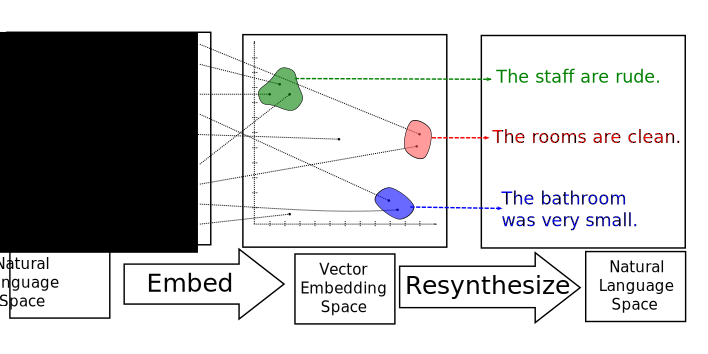
\includegraphics[scale=0.5]{workflow}
\end{frame}

\begin{frame}{Why are we converting SOWE to BOW?}
	\begin{itemize}
		\item<1-> Part-way step towards sentence generation.
		\item<2-> Translating various media to keywords via common vector space.
		%\iitem{This lets some classical IR methods be combine in with vector methods.}
		\item<3-> Theoretical implications on what information is maintained by the SOWE.
		
	\end{itemize}
\end{frame}



\begin{frame}{We have turned sentences into numeric vectors, now we want to turn them back.}

	\begin{description}
		\item<1->[Sentence:] It was the best of times, it was the worst of times
		\item<2->[Vector representation:]  $[−0.79, 1.27, 0.28, ..., −1.29]$
		\item<3->[BOW output:] \texttt{\{best: 1,times: 2, worst: 1, \\it: 2, of: 2, the: 2, was: 2,, : 1\}}
		\vfill
		\item<4->[Sentence:] It was the worse of times, it was the best of times
	\end{description}
\end{frame}



\begin{frame}{Existing methods do not produce closely matching sentences.}
	\begin{itemize}
		\vfill
		\item Iyyer et al's compositional method
		\item Bowman et al's RNN based method
		\vfill
		\item<2-> Both are demonstrated to produce loosely similar sentences.
		\item<3-> Neither has show a demonstration on any large scale corpus.
		\vfill
		%\item<3-> This is a challenging problem
		%\iitem we the problem is made simpler if the ordering requirement is removed.
	\end{itemize}
	\footfullcite{iyyer2014generating}
	\footfullcite{Bowman2015SmoothGeneration}
	
\end{frame}



\newcommand{\blockdiagram}{
	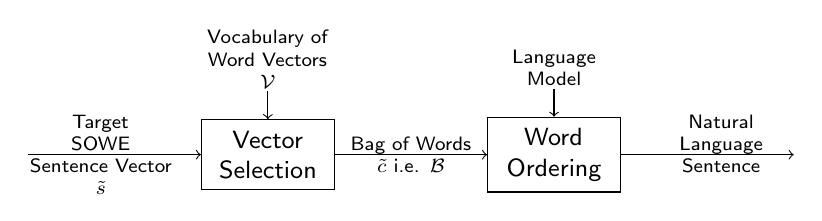
\begin{tikzpicture}[
	every node/.style={ text width=6em,
		align=center,
		font=\scriptsize\sffamily,
		inner sep=1pt
	},
	proc/.style= {draw,
		font=\small\sffamily,
		inner sep = 4pt,
		text width=4em
	}
	]
	\onslide<1,3->{
		\node (input) [inner sep=-4pt] {Target \\ SOWE\\ Sentence Vector\\ $\s$};
		\node (selection) [proc, right = 1em of input]{Vector\\ Selection};
		\node (vocab) [above = 1em of selection]{Vocabulary of Word Vectors \\ $\V$};
		\draw[->] (input.west) -- (selection);
		\draw[->] (vocab) -- (selection);
	}
	\onslide<2->{
		\node (ordering) [proc, right = 5.5em of selection]{Word\\ Ordering};
	}
	
	
	\draw[->] (selection) -- (ordering) node[midway] {Bag of Words\\ $\c$ i.e. $\B$ };
	\onslide<2,3->{
		\node (output) [inner sep=-4pt, right=1em of ordering] {Natural \\Language \\Sentence\\\null{ }};
		\node (lm) [above = 1em of ordering] {Language \\ Model};
		\draw[->] (lm) -- (ordering);
		\draw[->] (ordering) -- (output.east);
		
	}
	\end{tikzpicture}
}


\newcommand{\vectorselectionproblemdefn}{Find the inclusion vector $\c=[c_1,c_2,...c_{|\V|}]\in\N_0^{|\V|}$ that for we have $\min d(\s,\sum_{\x_j\in\V}\:\x_{j}\,c_{j})$}


\begin{frame}<1>{We solve the objective function to get a bag of words.}
	\vectorselectionproblemdefn
	\vfill
	\blockdiagram{}
	\vfill
\end{frame}


\begin{frame}[fragile]{We solve the objective function to get a bag of words.}
	\vectorselectionproblemdefn
	\vfill
	\begin{description}
		%\item<1->[Target Output] It was the best of times, it was the worst of times
		\item<2->[Input Vector]  $\s=[−0.79, 1.27, 0.28, ..., −1.29]$
		\vfill
		\item<3->[Vector Selection] 
		\begin{equation*}
		\s \approx \begin{array}{ll}
		&1\times[−0.19, 0.50, 0.14, ..., −0.59]\\
		+&2\times[-0.15, 0.19, 0.03, ..., -0.17]\\
		+&\qquad...\\
		+&0\times[−0.19, 2.10, 1.34, ..., 1.20]\\
		+&1\times[−0.79, 1.27, 0.28, ..., −1.29]\\
		\end{array}
		\end{equation*}
		\vfill
		\item<4->[BOW] \texttt{\{best: 1,times: 2, worst: 1, \\it: 2, of: 2, the: 2, was: 2,, : 1\}}
	\end{description}
	\vfill

\end{frame}

\begin{frame}{How to solve the objective function? Greedily}
	\vectorselectionproblemdefn
		\vfill
	\begin{itemize}
		\item<1-> Similarities to Knapsack family of problems.
		\iitem{Provably NP-Hard} \note{Can reduce to it from subset sum}
		\item<2-> Very high dimensionality of inclusion vector
		\begin{itemize}
			\item $|\V|\approx40,000$ for Brown Corpus
			\item $|\V|\approx180,000$ for Books Corpus
			\end{itemize}
		\item<3-> A greedy algorithm is linear time in $|\V|$ 
	\end{itemize}
	\vfill
\end{frame}

\newcommand{\vectorselectionproblemdefnalt}{Find the bag of vectors $\B$ (a multi-subset of $\V$), such that we have  $\min d(\s,\sum_{\x_a\in\B}\x_a)$}

\begin{frame}{A more direct bag notation for vector selection problem.}
	Rather than writing:\\
		\vectorselectionproblemdefn
	\vfill
	\note{This notation is good if you want to see how it is knapsack-like, for proving the reduction}
	\pause
	We can equivalently say:\\
		\vectorselectionproblemdefnalt
	\vfill
	\note{Note that he bag $\B$ has the inclusion vector $\c$, giving the multiplicity of each element of $\V$}

	
\end{frame}


\begin{frame}{Greedy Addition: where you add the best vector to your current bag, and repeat.}
	\vectorselectionproblemdefnalt
	\vfill
	\begin{enumerate}
		\item For each vector $\x_j$ in the vocabulary consider  $d(\s, \Sigma(\B)+\x_j)$
		\item Add in the vector that gets the total closest to $\s$ $\B\leftarrow\B\cup\{\x_\star\}$
			\begin{itemize}
				\item unless adding nothing would be better -- then terminate
			\end{itemize}
		\item Repeat
	\end{enumerate}
	\vfill
\end{frame}

\begin{frame}{A 1 dimentional example of greedy additon}
	\vectorselectionproblemdefnalt
	\vfill
	Consider $\V=\{24,25,100\}$ \hfill $\s=148$ \hfill $d(x,y)=|x-y|$
	\begin{enumerate}
		\item<1-> $\B=[\:]$ \hfill $d(\s,\Sigma(\B))=|148-0|=148$ 
		\item<2-> $\B=[100]$ \hfill $d(\s,\Sigma(\B))=|148-100|=48$ 
		\item<3-> $\B=[100,25]$ \hfill $d(\s,\Sigma(\B))=|148-(100+25)|=23$ 
		\item<4-> $\B=[100,25,24]$ \hfill $d(\s,\Sigma(\B))=|148-(100+25+24)|=1$ 
		\item<5-> $\B=[100,25,24]$ \hfill No improvement possible \hfill $d(\s,\Sigma(\B))=1$ 
	\end{enumerate}
	\vfill
	\onslide<6->{Fell for greedy trap}
	\vfill
	\note{If we knew the other elements of the bag would be 100, and 24 then we would not have put in a 25}
\end{frame}

\begin{frame}{1-Subsitution: Lessen the greed by reconsidering past choices}
	\vectorselectionproblemdefnalt
	\vfill
	\begin{enumerate}
		\item Consider each word vector in the current bag $\x_a\in\B$
		\item Would deleting it improve the score? $d(\s,\Sigma(\B)-\x_a)<d(\s,\Sigma(\B))$ ?
		\item Can it be swapped for another word to improve the score?
		$\exists \x_b\in\V$ such that
		$d(\s,\Sigma(\B)-\x_a+\x_b))<d(\s,\Sigma(\B))$ ?
	\end{enumerate}
\end{frame}

\begin{frame}{A 1 dimentional example of 1-substitution}
	\vectorselectionproblemdefnalt
	\vfill
	Consider $\V=\{24,25,100\}$ \hfill $\s=148$ \hfill $d(x,y)=|x-y|$
	\begin{enumerate}
		\item<1-> $\B=[100,25,24]$ \hfill $d(\s,\Sigma(\B))=|148-(100+25+24)|=1$
		
		\item<2-> Consider swapping $100$
		\item<3-> Consider swapping $25$
		\item<4-> $\B=[100,24,24]$ \hfill $d(\s,\Sigma(\B))=|148-(100+24+24)|=0$ 
		%\item<5-> Consider swapping $24$
	\end{enumerate}
	\vfill
	\onslide<5->{Fixed, but there are deeper greedy traps, that can be constructed.}
	\vfill
\end{frame}


\begin{frame}{Run until converance}
	\vfill
	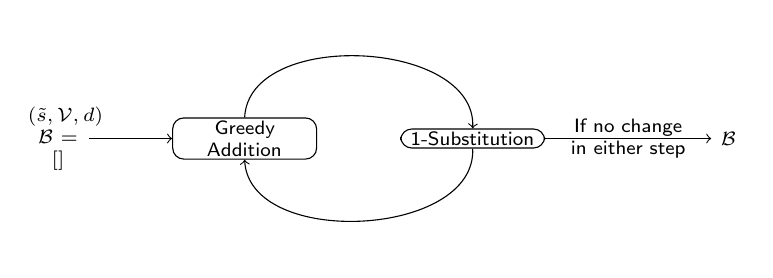
\begin{tikzpicture}[
		every node/.style={ text width=5em,
			align=center,
			font=\scriptsize\sffamily,
			inner sep=1pt,
		},
		]

		\node (input) [text width=2em] {$(\s,\V,d)$\\$\B=[]$};
		\node (addition) [draw, rounded corners, right = 3em of input]{Greedy Addition};
		\node (substitution) [draw, rounded corners, right = 3em of addition]{1-Substitution};
		\node (output) [right = 6em of substitution,text width=1em] {$\B$};
		\draw[->] (input) -- (addition);
		\path[->] (addition) edge [bend left=90,looseness=1] (substitution);
		\path[->] (substitution) edge [bend left=90,looseness=1] (addition);
		\draw[->] (substitution) -- (output) node[midway] {If no change in either step};
			
	\end{tikzpicture}
		\vfill
\end{frame}


\section{Experimental Setup}

\begin{frame}{Preprocess corpora to only use known words.}
	\begin{itemize}
		\item<1-> For word embeddings, we use pretrained GloVe \footfullcite{pennington2014glove}
		\item<2-> Restrict vector vocabulary to only words used in corpora
		\item<3-> Preprocess corpora to remove sentences with words not found in vocabulary.
	\end{itemize}
\end{frame}

\begin{frame}{We used the Brown, and the Books Corpus as generation targets.}
	\footfullcite{francis1979brown}
	\footfullcite{moviebook}
	\pause
	\begin{columns}[T]
		\begin{column}{0.5\textwidth}
			\textbf{\textcolor{darkbrown}{Brown Corpus}}
			\begin{itemize}
				\item Extracts from 500 varied works from 1961
				\item 40,485 unique words
				\item 42,004 sentences
				\item Sentence Length Q3: \\\hfill 25 words
			\end{itemize} 
		\end{column}
		\begin{column}{0.5\textwidth}
			\pause
			\textbf{\textcolor{darkbrown}{Books Corpus}}
			\begin{itemize}
				\item 11,038 unpublished novels\\we use a random subset
				\item 178,694 unique words
				\item 66,464 sentences 
				\item Sentence Length Q3: \\\hfill 17 words
			\end{itemize}
		\end{column}
	\end{columns}

\end{frame}


\section{Results}

\begin{frame}{A pair of short example}
	\vfill
	\begin{description}
		\item[Sentence:] we looked out at the setting sun .
		\item[Target BOW:]  . at looked out setting sun the we
		\item[Output BOW:]  . at looked out setting sun the we 
		\vspace{0.5cm}
		\item[Bowman et al's:] they were laughing at the same time .
	\end{description}
	\vfill
\end{frame}
\begin{frame}{A pair of short example}
	\vfill
	\begin{description}
		\item[Sentence:] i went to the kitchen .
		\item[Target BOW:] . i kitchen the to went
		\item[Output BOW:] . i kitchen the to went 
		\vspace{0.5cm}
		\item[Bowman et al's:] i went to the kitchen . 
	\end{description}
	\vfill
	\footfullcite{Bowman2015SmoothGeneration}
\end{frame}

\begin{frame}[fragile]{A short example where the method fails}
	
	\begin{description}
		\let\oldtextbf\textbf
		\renewcommand{\emph}[1]{\textcolor{blue}{\oldtextbf{#1}}}
		\renewcommand{\textbf}[1]{\textcolor{red}{\cancel{#1}}}
		\item[Sentence:] how are you doing ?
		\item[Target BOW:] ? are doing how you
		\item[Output BOW:] ? \emph{'re} \textbf{are} \emph{do} \textbf{doing} how  \emph{well} \textbf{you}
		\vspace{1cm}
		\item[Bowman et al's:] what are you doing ?
		
	\end{description}
	\footfullcite{Bowman2015SmoothGeneration}	
\end{frame}


\begin{frame}{A medium length example}
	\begin{description}
		\item[Sentence:] this is the basis of a comedy of manners first performed in 1892
		\item[Target BOW:] 1892 a   basis   comedy  first   in  is  manners of  of  performed   the this
		\item[Output BOW:] 1892 a   basis   comedy  first   in  is  manners of  of  performed   the this   
		\vspace{1cm}
		\item[Iyyer et al's] another is the subject of this trilogy of romance most performed in 1874
	\end{description}
	\footfullcite{iyyer2014generating}
\end{frame}


\begin{frame}{A long example}
	\begin{description}
		\item[Sentence:] thus she leaves her husband and child for aleksei vronsky but all ends sadly when she leaps in front of a train
		\item[Target BOW:] a    aleksei all and but child   ends    for front   her husband in  leaps   leaves  of  sadly   she she thus    train   vronsky when
		\item[Output BOW:] a    aleksei all and but child   ends    for front   her husband in  leaps   leaves  of  sadly   she she thus    train   vronsky when
		\vspace{1cm}
		\item[Iyyer et al's:] however she leaves her sister and daughter from former fianc\'e and she ends unfortunately when narrator drives into life of a house 
	\end{description}
	\footfullcite{iyyer2014generating}
\end{frame}

\begin{frame}[fragile]{A long example where the method fails.}
	\begin{description}
		\let\oldtextbf\textbf
		\renewcommand{\textbf}[1]{\textcolor{blue}{\oldtextbf{#1}}}
		\renewcommand{\emph}[1]{\textcolor{red}{\cancel{#1}}} %Note: Opposite from before
		\item[Sentence:] ralph waldo emerson dismissed this poet as the jingle man and james russell lowell called him three-fifths genius and two-fifths sheer fudge
		\item[Target BOW:] and  and  as  called  dismissed  emerson  fudge  genius  him  james  jingle  lowell  man  poet  ralph  russell  sheer  the  this  three-fifths  two-fifths  waldo
		\begin{overprint}
			\only<1>{
				\item[Output BOW:] \textbf{2008}   \textbf{\_...\_(13)}   \textbf{\_...\_(34)}   \textbf{\_...\_(44)}  \textbf{``}   \textbf{aldrick}   and and  \emph{as}   \textbf{both}   called   dismissed   emerson   fudge   genius   \textbf{hapless}   him   \textbf{hirsute}   james   jingle   \textbf{known}   lowell   man   poet   ralph   russell   sheer   the   this   three-fifths   two-fifths   waldo   \textbf{was}}
			
			\only<2>{
				\vspace{1cm}
				\item[Iyyer et al's:] henry\_david\_thoreau rejected this author like the tsar boat and imbalance created known good writing and his own death 
				}
		\end{overprint}
 
		
	\end{description}
	\footfullcite{iyyer2014generating}
\end{frame}





\begin{frame}{Yet another example}
	\begin{description}
		\item[Sentence:] in a third novel a sailor abandons the patna and meets marlow who in another novel meets kurtz in the congo
		\item[Target BOW:] a    a   abandons    and another congo   in  in  in  kurtz   marlow  meets   meets   novel   novel   patna   sailor  the the third   who
		\item[Output BOW:] a    a   abandons    and another congo   in  in  in  kurtz   marlow  meets   meets   novel   novel   patna   sailor  the the third   who
		\vspace{1cm}
		\item[Iyyer et al's:] during the short book the lady seduces the family and meets cousin he in a novel dies sister from the mr.
	\end{description}
	\footfullcite{iyyer2014generating}
\end{frame}

\begin{frame}{A final example}
	\begin{description}
		\item[Sentence:] name this 1922 novel about leopold bloom written by james joyce
		\item[Target BOW:] 1922 about   bloom   by  james   joyce   leopold name    novel   this    written
		\item[Output BOW:] 1922 about   bloom   by  james   joyce   leopold name    novel   this    written
		\vspace{1cm}
		\item[Iyyer et al's:] name this 1906 novel about gottlieb\_fecknoe inspired by james\_joyce
	\end{description}
	\footfullcite{iyyer2014generating}
\end{frame}



\pgfplotstableread[col sep=comma,header=has colnames]{../data/selection_overall_len_scores.csv}{\seloverallscores}

\begin{frame}{Results: The more dimentions used in the word embeddings, the better the recovery.}
	\begin{tikzpicture}
	\begin{axis}[ybar, bar width=1cm,
	ylabel=Portion Perfect,
	yticklabel=\pgfmathparse{100*\tick}\pgfmathprintnumber{\pgfmathresult}\,$\%$,
	yticklabel style={/pgf/number format/.cd,fixed,precision=2},
	ymin=0,ymax=1,
	xticklabels = {.,Brown\\50d,Brown\\100d,Brown\\200d,Brown\\300d,Books\\300d},
	xticklabel style={align=center}
	]
	\addplot table [y=Portion Perfect, x expr=\coordindex] {\seloverallscores};
	
	\end{axis}
	\end{tikzpicture}
\end{frame}

\begin{frame}{Results: The more dimentions used in the word embeddings, the better the recovery.}
	\begin{tikzpicture}
	\begin{axis}[ybar, bar width=1cm,
	ylabel=Mean Jaccard Index,
	yticklabel=\pgfmathparse{100*\tick}\pgfmathprintnumber{\pgfmathresult}\,$\%$,
	yticklabel style={/pgf/number format/.cd,fixed,precision=2},
	ymin=0, ymax=1,
	xticklabels = {.,Brown\\50d,Brown\\100d,Brown\\200d,Brown\\300d,Books\\300d},
	xticklabel style={align=center}
	]
	\addplot[fill=brown!50!chamois, draw=brown] table [y=Mean Jaccard Score, x expr=\coordindex] {\seloverallscores};
	
	\end{axis}
	\end{tikzpicture}
\end{frame}



\begin{frame}{}
	\only<1>{\frametitle{Result: The longer the sentence, the worse recovery}}
	\only<2>{\frametitle{Result: The larger the vocabulary, the worse recovery}\topline}
	
	\pgfplotstableread[col sep=comma,header=has colnames]{../data/selection_len_scores.csv}{\sellenscores}
	
	\begin{tikzpicture}
	\begin{axis}[xlabel=Ground Truth Sentence Length,
	ylabel=Mean Jaccard Index,
	cycle list name=exotic]
	\addplot table [y=books_0_01_glove300_jaccard_mean,x=ground_len]{\sellenscores};
	\addplot table [y=brown_glove300_jaccard_mean,x=ground_len]{\sellenscores};%
	\only<1>{
		\addplot table [y=brown_glove200_jaccard_mean,x=ground_len]{\sellenscores};
		\addplot table [y=brown_glove100_jaccard_mean,x=ground_len]{\sellenscores};
		\addplot table [y=brown_glove50_jaccard_mean,x=ground_len]{\sellenscores};}

	\legend{300D Books, 300D Brown, 200D Brown,100D Brown, 50D Brown}					
	\end{axis}
	\end{tikzpicture}	
	
	\alert{
	\only<1>{Brown Q3: 25 words \hfill Books Q3: 17 words}
	\only<2>{Brown $|\V|\approx40,000$ \hfill Books $|\V|\approx180,000$}
	}
\end{frame}


\section{Conclusion}

\begin{frame}{Future Work: we could to order them to get a sentence.}
	\begin{itemize}
		\item<1-> Use a language model to find probability of any given sequence.
		\item<2-> Not guaranteed to find a single unique order.
		\item<3-> Also NP-hard.
	\end{itemize}
	
\end{frame}

\begin{frame}<1,3>{A two step method for generating sentences.}
	\blockdiagram
\end{frame}

\begin{frame}{Conclusion: We can often successfully recover the BOW, from the SOWE}
	\begin{itemize}
		\item Vector selection with a greedy algorithm
		\begin{itemize}
			\item This is a broad generalisation of Knapsack Problem
			\item Input: SOWE vector
			\item Greedy Addition + 1-Substitution til convergence.
			\item Output: BOW
		\end{itemize}
		\vfill
		\item Future work: order the words using a language model. 
	\end{itemize}
\end{frame}


\section{Appendix}

\begin{frame}{Recent results suggest sum of word embeddings captures surprising amounts of semantic information}
	\vskip1.5ex
	\scriptsize
	\begin{tabular}{cc}
		Category & Example\\
		\hline
		Adhesion to Vertical Surface & There is a magnet on the refrigerator.\\
		Support by Horizontal Surface & There is an apple on the refrigerator.\\
		Support from Above & There is an apple on the branch.\\
		Full Containment & There is an apple in the refrigerator.\\
		Partial Containment & There is an apple in the water. 
	\end{tabular}
	\normalsize
	\vfill
	\begin{itemize}
		\item Categorise sentences based on the positional component of their meaning.
		%\item This is challenging as it is word overlap independent.
		\item Ritter et. al. found sum of word embeddings to outperform all more complex models.
	\end{itemize}
	\footfullcite{RitterPosition}
\end{frame}

\begin{frame}{Recent results suggest sum of word embeddings captures surprising amounts of semantic information}
	\begin{itemize}
		\item We groups MSRP and Opinosis sentences by semantic equivalence forming classes of paraphrases.
		\item Then used various sentence embeddings as input to a linear SVM to try and classify back into the groups.
		\item SOWE was amongst top contenders (<0.6\% worse than best in both cases)
	\end{itemize}
	\footfullcite{White2015SentVecMeaning}
\end{frame}


\begin{frame}{Iyyer et al's compositional sentence generation method.}
	\footfullcite{iyyer2014generating}
	\begin{itemize}
		\item Variation on the URAE
		\item Reuses a neural network to (merge up the dependency tree
		\item Similar to unfold.
		\item Requires structure of output to be given as a input.
	\end{itemize}
\end{frame}


\begin{frame}{Bowman et al's RNN based sentence generation method.}
	\footfullcite{Bowman2015SmoothGeneration}
	\begin{itemize}
		\item Use LTSM RNN for decode/encoding step
		\item Use VAE as representation of posterior probabilities. 
		\item lots of interesting properties and other uses.
	\end{itemize} 
\end{frame}

\begin{frame}{Results}
	\begin{table}
		\pgfplotstabletypeset[col sep=comma,fixed zerofill, precision=3,column type=C{3em},
		columns/Corpus/.style={string type},
		columns/Word Embedding Dimensions/.style={string type},
		columns/Portion Perfect/.style={percent style, precision=1},
		columns/Mean Jaccard Score/.style{name=Mean Jacard Index}
		every head row/.style={
			after row=\midrule
		}]{../data/selection_overall_len_scores.csv}
	\end{table}
\end{frame}


\end{document}